\chapter{Synthese}\label{synthese}

Die Untersuchungen in Kapitel \ref{analyse} haben gezeigt, dass die existierenden untersuchten Verfahren nicht ausreichend sind, um die Qualität von \ac{BKG}-Signal aus Langzeitaufnahmen von Patient*innen zu beurteilen. Deshalb werden weitere Möglichkeiten zu diesem Zweck untersucht und der Fokus dabei vor allem auf die Konstruktion und Analyse der Eingabemerkmale gelegt. Es wird eine Auswahl von Modellen zum Testen getroffen und ein Basisklassifikator zum Vergleich dieser Modelle entwickelt.

\section{Merkmalskonstruktion}

Grundsätzlich muss zwischen zwei Eingabeformen unterschieden werden: Der bisher betrachteten Eingabe von Merkmalen und die Eingabe des Signals selbst. Letzteres hat den Vorteil, dass keine Informationen verloren gehen können. Allerdings ist das Training so sehr rechen- und damit auch zeitaufwändig und die Merkmale, die zur Beurteilung der Signalqualität genutzt werden sind nur schwer nachvollziehbar. Aus diesen Gründen wird in dieser Arbeit die Eingabe von Merkmalen untersucht.

Neben der Konstruktion von neuen Merkmalen können ebenfalls die Ergebnisse aus Kapitel \ref{analyse} verwendet werden, das bedeutet das reduzierte Set statistischer Merkmale und der \ac{SQI} des \ac{CLIE}-Algorithmus, bzw. die Coverage durch Intervalle, deren \ac{SQI} über einem Schwellwert $q\textsubscript{th}$ liegt. Das Vorgehen bei der Konstruktion neuer Merkmale besteht darin, diese zunächst zu sammeln und anschließend zu untersuchen, Zusammenhänge zu ermitteln und mit den gewonnenen Erkenntnisse die Merkmale zu reduzieren und in Relation zueinander zu setzen.

Da die Untersuchung in Kapitel \ref{eval-brueser} gezeigt hat, dass die Ergebnisse stark abhängig von der Auswahl des Schwellwerts $q\textsubscript{th}$ für den \ac{SQI} sind, wurde die Coverage für die Schwellwerte $q\textsubscript{th} = 0.3$, $q\textsubscript{th} = 0.4$ und $q\textsubscript{th} = 0.5$ als Merkmal ausgewählt. Da die Verteilung des \ac{SQI} auf dem Segment womöglich weitere Erkenntnisse ermöglicht, wurden außerdem Merkmale zu der Verteilung der \ac{SQI} aller ermittelten Intervalle berechnet:
\begin{itemize}
	\item Minimum $\text{SQI}\textsubscript{min}$
	\item Maximum $\text{SQI}\textsubscript{max}$
	\item Standardabweichung $\text{SQI}\textsubscript{std}$
	\item Mittelwert $\text{SQI}\textsubscript{mean}$
	\item Median $\text{SQI}\textsubscript{median}$
\end{itemize}

Auch die geschätzten Intervalllängen können womöglich Aufschluss über die Signalqualität geben. Hier muss allerdings auch beachtet werden, dass dadurch auch die Gefahr von physiologischen Einschränkungen besteht, was \acl{HR} und \acl{HRV} betrifft, wenn die Trainingsdaten nicht variabel genug sind, sodass medizinische Abnormalitäten als Signal schlechter Qualität eingeordnet werden. Es muss also bei einer Verwendung geprüft werden, wie diese Werte einbezogen werden. Die serialisierten Merkmale mit Bezug auf die geschätzten Intervalllängen sind:

\begin{itemize}
	\item Mittelwert $\text{IL}\textsubscript{mean}$
	\item Spannweite $\text{IL}\textsubscript{range}$
	\item Standardabweichung $\text{IL}\textsubscript{std}$
\end{itemize}

Bei \ac{PPG}-Signalen verwenden \citeauthor{Yu2020} erfolgreich herzratenbezogene Merkmale, indem die maximale Frequenz des Spektogramms der Autokorrelation über das Segment berechnet wird und in Verhältnis zur geschätzten Herzrate gesetzt wird.\footcite{Yu2020} Sei $f\textsubscript{ACF}$ die maximale Frequenz und $f\textsubscript{HR}$ die Frequenz der geschätzten Herzrate, werden zwei Merkmale daraus abgeleitet:
\begin{itemize}
 	\item $\texttt{ratio}\textsubscript{ACF} = \frac{f\textsubscript{HR}}{f\textsubscript{ACF}}$
 	\item $\texttt{diff}\textsubscript{ACF} = f\textsubscript{HR} - f\textsubscript{ACF}$
\end{itemize}
 
 Da auch das Spektogramm der gefilterten Daten des Segments Informationen liefern kann, wurden diese Merkmale analog mit der maximalen Frequenz der Daten $f\textsubscript{data}$ berechnet:
 \begin{itemize}
 	\item $\texttt{ratio}\textsubscript{data} = \frac{f\textsubscript{HR}}{f\textsubscript{data}}$
 	\item $\texttt{diff}\textsubscript{data} = f\textsubscript{HR} - f\textsubscript{data}$
 \end{itemize}

Bei weiteren Merkmalen wird versucht, die Eigenschaft der Selbstähnlichkeit zu beschreiben. Dafür werden zunächst die Hochpunkte betrachtet, an denen der \ac{CLIE}-Algorithmus die Herzschläge verortet. Von diesen werden folgende Merkmale serialisiert:
\begin{itemize}
	\item Spannweite $\text{P}\textsubscript{range}$
	\item Mittelwert $\text{P}\textsubscript{mean}$
	\item Standardabweichung $\text{P}\textsubscript{std}$
\end{itemize}

In weiteren Merkmalen wird versucht, die Selbstähnlichkeit durch statistische Merkmale zu erfassen. Hierzu wird von den vom \ac{CLIE}-Algorithmus erkannten Herzschläge jeweils Mittelwert, Standardabweichung und Spannweite berechnet. Von dieser Menge an Intervallen wird jeweils die Standardabweichung als Merkmal extrahiert, um die Variation über das Segment einzufangen:
\begin{itemize}
	\item Standardabweichung alle Mittelwerte $\texttt{mean}\textsubscript{std}$
	\item Standardabweichung aller Spannweiten $\texttt{range}\textsubscript{std}$
	\item Standardabweichung aller Standarabweichungen $\texttt{std}\textsubscript{std}$
\end{itemize}

Häufig werden für die Beurteilung von Signalqualität Templates verwendet. Bei \ac{BKG}-Signalen werden diese durch beispielsweise Positionsänderungen obsolet, allerdings entspricht ein Segment nur einem sehr kurzen Zeitraum, weshalb Templates in diesem Fall verwendet werden können. Es werden zwei verschiedene Templates betrachtet: Zunächst das geschätzte Schlag-zu-Schlag-Intervall mit dem höchsten \ac{SQI}, $T\textsubscript{SQI}$ genannt, und der Herzschlag mit der mittleren Intervalllänge, $T\textsubscript{median}$, dessen Länge auch für die Schätzung der Herzrate verwendet wird. Es werden beide betrachtet, da ein sehr hoher \ac{SQI} auch bei rhythmischen Artefakten auftreten kann. Zu diesen beiden Templates wird für jeden geschätzten Herzschlag die Kreuzkorrelation berechnet. Von dieser Menge an Korrelationen wird jeweils Mittelwert und Standardabweichung als Merkmal verwendet:
\begin{itemize}
	\item $\texttt{mean}\textsubscript{T\textsubscript{median}}$
	\item $\texttt{std}\textsubscript{T\textsubscript{median}}$
	\item $\texttt{mean}\textsubscript{T\textsubscript{SQI}}$
	\item $\texttt{std}\textsubscript{T\textsubscript{SQI}}$
\end{itemize}

Außerdem wird die absolute Energie des Segmentes berechnet:
\begin{itemize}
	\item $E\textsubscript{abs} = \sum_t s(t)^2$
\end{itemize}

Da die Berechnung aller Merkmale für die Menge der Daten zeit- und rechenaufwändig ist, werden diese einmalig berechnet und anschließend in einer csv-Datei gespeichert.

\section{Explorative Datenanalyse und Merkmalsreduktion}

Durch die Extraktion mehrerer Merkmale pro betrachteter Eigenschaft entstehen korrelierte Merkmale, bei denen es nötig ist, sie zu reduzieren oder zusammenzufassen. Dies geschieht im Zuge der explorativen Datenanalyse. Die Korrelationen sind in dem erzeugten Korrelationsdiagramm, das in Abbildung \ref{fig:corr-heatmap-own} gezeigt ist, deutlich sichtbar.

\begin{figure}[H]
	\centering
	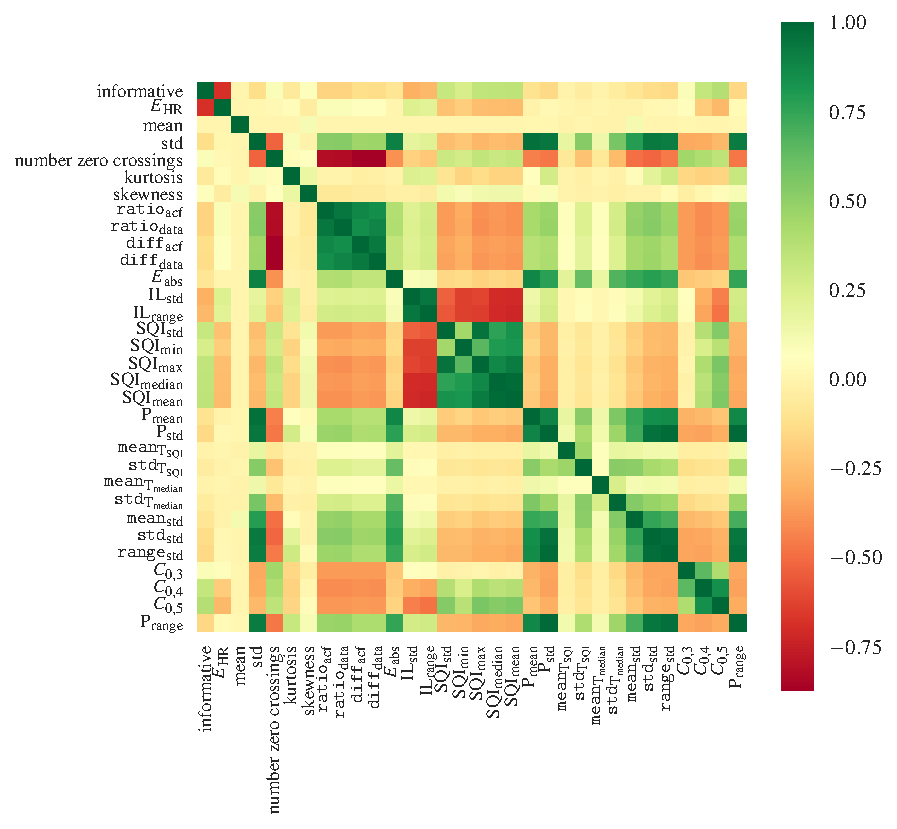
\includegraphics{pic/corr-heatmap-own.pdf}
	\caption{Korrelationsdiagramm aller entwickelten Merkmale, $E\textsubscript{HR}$ und der binären Annotation}
	\label{fig:corr-heatmap-own}
\end{figure}
 
Auch bei diesen Merkmalen wird mit dem Python-Paket \texttt{rfimp} ermittelt, welche Merkmale durch andere vorhergesagt werden können. Im Zuge der Merkmalskonstruktion werden Merkmale verworfen, die sich durch ein einzelnes anderes Merkmal vorhersagen lassen.

Es zeigt sich, dass Standardabweichung und Spannweite der Werte jeweils die Vorhersage des anderen Wertes ermöglichen. Aus diesem Grund werden $\texttt{P}\textsubscript{range}$, $\texttt{range}\textsubscript{std}$ und $\text{IL}\textsubscript{range}$ als Merkmale verworfen. Das gleiche gilt für $\text{SQI}\textsubscript{max}$. Auch bietet $E\textsubscript{abs}$ keinen Mehrgewinn zu der Standardabweichung des Segments. Die Merkmale $\texttt{ratio}\textsubscript{acf}$ und $\texttt{diff}\textsubscript{acf}$ sind durch ihre Definition stark miteinander korreliert und da die Untersuchung zeigt, dass $\texttt{diff}\textsubscript{acf}$ schlechter vorhergesagt werden kann, wird $\texttt{ratio}\textsubscript{acf}$. Das gleiche gilt für $\texttt{ratio}\textsubscript{data}$. Wie zu erwarten war, sind auch $\text{SQI}\textsubscript{median}$ und $\text{SQI}\textsubscript{mean}$ stark korreliert. Die mit \texttt{rfpimp} berechneten Abhängigkeiten zeigen. dass dar Median schlechter vorhergesagt werden kann, weshalb $\text{SQI}\textsubscript{mean}$ verworfen wird.

Nach Reduktion um diese Merkmale wird die Berechnung der Abhängigkeiten wiederholt. Es zeigen sich weitere Abhängigkeiten zwischen $\texttt{P}\textsubscript{mean}$ und der Standardabweichung und $\texttt{std}\textsubscript{std}$ und $\texttt{P}\textsubscript{std}$, weshalb Standardabweichung und $\texttt{std}\textsubscript{std}$ verworfen werden. Keine der erkannten Abhängigkeiten ist unerwartet. Dieser Prozess erlaubt jedoch, vermutete Abhängigkeiten zu bestätigen und die Merkmale zu verwenden, die einen höheren Informationsgehalt haben.

Die verbleibenden 21 Merkmale

\section{Auswahl der Modelle und Aufbau eines Basisklassifikators}

Nachdem die Merkmale entwickelt sind, werden nun Modelle ausgewählt, mit denen die Untersuchung durchgeführt wird.

Die Auswahl beschränkt sich auf zwei Modelle, den \acl{RF} und den Gradient Boosting Tree. Beide sind ein Ensemble aus schwächeren \ac{CART}s und ermöglichen schnell trainierende, robuste Modelle, deren Entscheidung sich leicht nachvollziehen lässt, und erzielen meist gute Ergebnisse. Dadurch wird eine Untersuchung der Merkmale, anhand derer die Signalqualität beurteilt werden kann, möglich.

Beide Modelle eignen sich sowohl für Regression als auch Klassifikation. Dies wird genutzt, um die Unterschiede der Ergebnisse und der Wichtigkeit der einzelnen Merkmale für beide Arten von Algorithmen zu vergleichen. Bei einer Regression kann der vorhergesagte Fehler $E\textsubscript{HR}$ mit einem Schwellwert in eine binäre Klassifikation umgewandelt werden. Dies ermöglicht einen einfachen Vergleich von Klassifikation und Regression. Damit ergeben sich insgesamt vier Lernmodelle: Jeweils Regression und Klassifikation mit einem \ac{RF} und einem Gradient Boosting Tree.

Um die Evaluation der verschiedenen Modelle zu vereinfachen, wird ein eigenständiges Basismodell entwickelt, dass das Laden der Daten, die Umwandlung der Regressionsergebnisse in eine binäre Klassifikation, das Hyperparameter-Tuning und die Evaluation der Ergebnisse bündelt.  Außerdem werden im Zuge dessen die Modelle nach dem Training serialisiert, um sie für eine  spätere Verwendung zu speichern. Dem Konstruktor dieses Basismodells werden Lernmodell, Dateiname zum Laden oder Speichern des Modells und die Hyperaramater, von denen die optimale Auswahl getroffen wird, übergeben. Wenn kein Lernmodell übergeben wird, wird automatisch versucht, die Datei mit dem übergebenen Namen zu laden. Optional kann eine Featureauswahl angegeben werden, die für das Modell verwendet werden soll. Des Weiteren werden die Eigenschaften des Datensets übergeben; das bedeutet die verwendete Segmentlänge, der Abstand in dem die Segmente erzeugt werden, und der verwendete Threshold. Wurde das Datenset noch nicht erzeugt, wird dies nachgeholt. 

Sind Hyperparameter angegeben, wird das Hyperparameter-Tuning mit einer Kreuzvalidierung auf dem Trainingsset durchgeführt, wobei jeweils ein*e Patient*in zum Testen ausgelassen wird. Bei dem Hyperparameter-Tuning für die statistischen Merkmale wurde die Accuracy optimiert. Da diese bei nicht balancierten Datensets an Aussagekraft verliert und nicht zwischen Falsch-Positiven und Falsch-Negativen unterscheidet, wird hier der F1-Score optimiert.

Da bei der Erzeugung der Merkmale Lücken entstehen können, wenn für das Segment keine Intervallschätzungen existieren, werden diese Segmente unabhängig von dem verwendeten Lernmodell als nicht informativ klassifiziert. Auch beim Training werden Datenpunkte, deren Merkmale lückenhaft sind, ausgeschlossen.

Das entwickelte Basismodell ermöglicht also Hyperparameter-Tuning, Training, Vorhersage und Evaluation. Damit können auch andere Modelle und andere Daten einfach untersucht werden.





